\documentclass{article}

\usepackage[margin=1in]{geometry}
\usepackage{tikz}
    \tikzstyle{hollow node} = [circle,draw,inner sep=1.5]
    \tikzstyle{solid node}  = [circle,draw,inner sep=1.5,fill=black]
    \usetikzlibrary{calc}
\usepackage{sgame}
    \gamemathtrue
\usepackage[shortlabels]{enumitem}
\usepackage{amsmath}

\author{Damien Prieur}
\title{Problem Set 6 \\ ECON 250}
\date{}

\begin{document}

\maketitle

\section{\emph{Ultra} and \emph{Soar}}
Two startups, \emph{Ultra} and \emph{Soar}, have developed fairly similar ridesharing apps and are competing for customers by deciding how much to advertise their app.
Let $A_{i} \ge 0$ be the advertising level of firm $i$.
The profits of each firm depend on how much it advertises its app but also on the advertising level of its opponent $A_{-i}$.
The higher the advertising levels the more visibility ridesharing apps and demand increases.
In particular, firm $i$'s profits are $u_{i}(A_{i},A_{-i}) = (90 + A_{i} + A_{-i})A_{i}-2A_{i}^{2}$.
\emph{Ultra} chooses $A_{1}$ first and, after observing it, \emph{Soar} chooses $A_{2}$.
\begin{enumerate}[(a)]
\item Draw the extensive form. Which are the proper subgames?
\newline
\begin{centering}
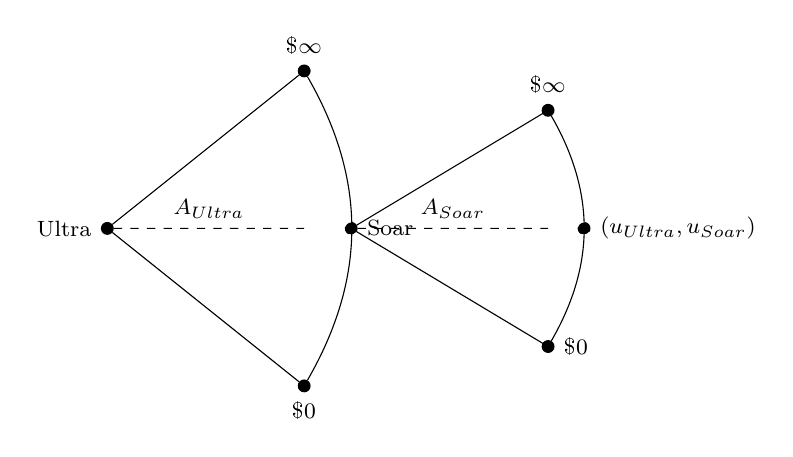
\begin{tikzpicture}[font=\footnotesize,
                    grow' = right
                    ]
\tikzstyle{level 1}=[level distance=25mm, sibling distance=20mm]
\tikzstyle{level 2}=[level distance=25mm, sibling distance=15mm]

    \node(0)[solid node, label=left:{Ultra}]{}
        % Upper part of arc
        child{node[solid node, label=above:{\$$\infty$}]{}}
        % Where y is chosen/offered, general case
        child{[dashed] node[solid node, xshift=17, label=right:{Soar}]{}
            child{[solid, black]  node(a)[solid node, label=above:{\$$\infty$}]{}}
            child{[dashed, black] node[solid node, xshift=13, label=right:{$(u_{Ultra},u_{Soar})$}]{} edge from parent node[above]{\textcolor{black}{$A_{Soar}$}}}
            child{[solid, black]  node(b)[solid node, label=right:{\$0}]{}}
            edge from parent node[above]{\textcolor{black}{$A_{Ultra}$}}
        }
        child{node[solid node, label=below:{\$0}]{}}
    ;

    \draw[bend left](0-1)to(0-3);
    \draw[bend left](a)to(b);


\end{tikzpicture}
\end{centering}
\newline
There is only one proper subgame as well as the full game above.
\newline
\begin{centering}
\begin{tikzpicture}[font=\footnotesize,
                    grow' = right
                    ]
\tikzstyle{level 1}=[level distance=25mm, sibling distance=20mm]
\tikzstyle{level 2}=[level distance=25mm, sibling distance=15mm]

    \node(0)[solid node, label=left:{Soar}]{}
        child{[solid, black]  node(a)[solid node, label=above:{\$$\infty$}]{}}
        child{[dashed, black] node[solid node, xshift=17, label=right:{$(u_{Ultra},u_{Soar})$}]{} edge from parent node[above]{\textcolor{black}{$A_{Soar}$}}}
        child{[solid, black]  node(b)[solid node, label=right:{\$0}]{}}
    ;

    \draw[bend left](a)to(b);


\end{tikzpicture}
\end{centering}

\item Find the SPNE. How does it compare to the NE of the simultaneous move game?
\newline
Looking at the smaller subgame they are best responding to when they maximize their utility $\frac{\delta u_{Soar}}{\delta A_{Soar}} = 0$
$$\frac{\delta u_{Soar}}{\delta A_{Soar}} = (90 + A_{Ultra} + A_{Soar}) + A_{Soar} - 4A_{Soar} = 90 + A_{Ultra} - 2A_{Soar} = 0$$
$$\implies A_{Soar} = \frac{90 + A_{Ultra}}{2}$$
Using backward induction we can find what Ultra should do solving the same equation but for their utility and Soar's choice filled in.
$$\frac{\delta u_{Ultra}}{\delta A_{Ultra}} = (90 + A_{Soar} + A_{Ultra}) + A_{Ultra} - 4A_{Ultra} = 90 + A_{Soar} - 2A_{Ultra} = 0$$
$$\implies A_{Ultra} = \frac{90 + A_{Soar}}{2} =  \frac{90 +  \frac{90 + A_{Ultar}}{2}}{2} \implies 4A_{Ultra} = 180 + 90 + A_{Ultra}$$
$$\implies A_{Ultra} = \frac{270}{3} = 90 $$
The SPNE will be $\sigma=(90, \frac{90 + A_{Ultra}}{2})$ Which is the same as for the simultaneous move game.


\item Is there a first-mover advantage in the market? Justify your answer.
\newline
No since the second player can punish the first player if they not according to the Nash equillibrium.
Also both players are getting the same reward so neither has an advantage.

\end{enumerate}

\section{\emph{Do it now or do it later}}
\emph{Do it now or do it later}. My friend Paco Vivalavida must do an activity \emph{only once} between now ($t = 1$) and $T = 4$.
That is, he has to choose a vector of decisions $(x_1,x_2,x_3,x_4), x_t \in {Y,N}$, where $x_t = Y$ means do the activity in period $t$ if he has not already don it at $t'<t$, and $x_t = N$ means not do the activity at $t$.
For instance, $(N,Y,N,Y)$ means Paco does not do the activity at $t = 1$, does the activity at $t = 2$ if it was not done before, does no do it at $t = 3$ if it has not been done before and does it at $t=4$ if it has not been done before.
Such a strategy leads to him actually doing the activity at $t = 2$.

\begin{itemize}
\item \emph{Rewarding Activity}. Paco loves movies and he just got a free movie ticket that he can use at the local movie theater in one of the next 4 Saturdays.
Each Saturday a different movie is shown, with better movies scheduled at later dates. In particular, Paco's (undiscounted) instantaneous utilities associated to each of the moves are $(u_1, u_2, u_2, u_4) = (3, 5, 8, 13)$, while he gets 0 if he does not watch a movie at $t$.
He has $\beta - \delta$ time preferences with $\delta=1$.
For instance, his utility at $t = 1$ from $(N,Y,N,Y)$ is $\beta u_2$ because he watches the 2nd-week movie, while he period-2 self derives utility $u_2$.
Similarly, his period-1 self gets $\beta u_4$ when he chooses $(N,N,N,Y)$ while he period-3 self gets $\beta u_4$.
[Hint: A useful way to visualize the decision problem is to draw a game tree in which an action $Y$ at period $t$ leads to a terminal node with payoff $u_t$, while an action $N$ leads to the next period decision node, except in the last period in which only action $y$ is available since he has to do the activity if he has not done so before.]
\begin{enumerate}[(a)]
\item If Paco's time preferences are given by $\beta = 1$, what is his optimal choice of $(x_1,x_2,x_3,x_4)$?
\newline
Paco's optimal choice is going to be $(N, N, N, Y)$ as for each $t_i$ where $i\in[1,3]$ he gets his time preference of $\beta u_4 = 13 $ and a final utility of $13$.

\item For the remainder of the problem assume Paco is present-biased with $\beta = 0.5$.
If he could commit to $(x_1, x_2, x_3, x_4)$ (e.g. by giving the coupon to a friend and instructing him to deliver it at a specific $t$), what would his choice be?
\newline
Not super sure how this differs from the next question.
\newline
His first choice would be to skip since the last two movies are interesting enough to overcome his present-bias.
In $t=2$ we are now only overcoming his present-bias due to $u_4$ so he will skip again.
When $t=3$ his present-bias will overcome the reward of the final movie so he will watch the movie at $t=3$.
When $t=4$ he has to watch the movie if he has not yet so this gives us:
\newline
$\sigma = (N,N,Y,Y) $
\newline
I think this is what it's asking for:
\newline
If he had to make a decision at $t=1$ then he would tell his friend to give it to him at $t=4$ as it has the highest utility after applying the present-bias.

\item If Paco is sophisticated, what would he choose?
Does he 'preproperate' (do an activity too soon)?
[Hint: draw the game tree and use backward induction, applying the discounting as we did in the alternating offers bargaining game.]
\newline
His first choice would be to skip since the last two movies are interesting enough to overcome his present-bias.
In $t=2$ we are now only overcoming his present-bias due to $u_4$ so he will skip again.
When $t=3$ his present-bias will overcome the reward of the final movie so he will watch the movie at $t=3$.
When $t=4$ he has to watch the movie if he has not yet so this gives us:
\newline
$\sigma = (N,N,Y,Y) $
\end{enumerate}
\end{itemize}

\end{document}
